\chapter{Builder模式}
\section{Builder模式的定义}
建造者(Builder)模式的定义:指将一个复杂对象的构造与它的表示分离,使同样的构建过程可以创建不同的表示,这样的设计模式被称为建造者模式。它是将一个复杂的对象分解为多个简单的对象,然后一步一步构建而成。它将变与不变相分离,即产品的组成部分是不变的,但每一部分是可以灵活选择的。
\subsection{优点}
\begin{enumerate}
	\item 各个具体的建造者相互独立,有利于系统的扩展。
	\item 客户端不必知道产品内部组成的细节,便于控制细节风险。
\end{enumerate}
\subsection{缺点}
\begin{enumerate}
	\item 产品的组成部分必须相同,这限制了其使用范围。
	\item 如果产品的内部变化复杂,该模式会增加很多的建造者类。
\end{enumerate}
注:
建造者(Builder)模式和工厂模式的关注点不同:建造者模式注重零部件的组装过程,而工厂方法模式更注重零部件的创建过程,但两者可以结合使用。
\subsection{应用场景}
\begin{itemize}
	\item 创建的对象较复杂,由多个部件构成,各部件面临着复杂的变化,但构件间的建造顺序是稳定的。
	\item 创建复杂对象的算法独立于该对象的组成部分以及它们的装配方式,即产品的构建过程和最终的表示是独立的。
\end{itemize}
\subsection{角色}
\begin{enumerate}
	\item 产品角色(Product):它是包含多个组成部件的复杂对象,由具体建造者来创建其各个滅部件。
	\item 抽象建造者(Builder):它是一个包含创建产品各个子部件的抽象方法的接口,通常还包含一个返回复杂产品的方法 getResult()。
	\item 具体建造者(Concrete Builder):实现 Builder 接口,完成复杂产品的各个部件的具体创建方法。
	\item 指挥者(Director):它调用建造者对象中的部件构造与装配方法完成复杂对象的创建,在指挥者中不涉及具体产品的信息。
\end{enumerate}
\section{建造者模式——例一}
\noindent 注:
\begin{enumerate}
	\item Director不关心实际编写文档的是TextBuilder还是HTMLBuilder。
\end{enumerate}
\begin{lstlisting}
//抽象建造者
public abstract class Builder {
	public abstract void makeTitle(String title);
	public abstract void makeString(String str);
	public abstract void makeItems(String[] items);
	public abstract void close();
}
\end{lstlisting}
\begin{lstlisting}
//Plain建造者
public class TextBuilder extends Builder {
	private StringBuffer buffer = new StringBuffer();
	public void makeTitle(String title) {
		buffer.append("========================\n");
		buffer.append("[" + title + "]\n");
		buffer.append("\n");
	}
	public void makeString(String str) {
		buffer.append("~" + str + "\n");
		buffer.append("\n");
	}
	public void makeItems(String[] items) {
		for (int i = 0; i < items.length; i++) {
			buffer.append(" ." + items[i] + "\n");
		}
		buffer.append("\n");
	}
	public void close() {
		buffer.append("========================\n");
	}
	public String getResult() {
		return buffer.toString();
	}
}
\end{lstlisting}
\begin{lstlisting}
//HTML建造者
public class HTMLBuilder extends Builder {
	private String filename;
	private PrintWriter writer;
	public void makeTitle(String title) {
		filename = title + ".html";
		try {
			writer = new PrintWriter(new FileWriter(filename));
		} catch (IOException e) {
			e.printStackTrace();
		}
		writer.println("<html><head><title>" + title + "</title></head><body>");
		writer.println("<h1>" + title + "</h1>");
	}
	public void makeString(String str) {
		writer.println("<p>" + str + "</p>");
	}
	public void makeItems(String[] items) {
		writer.println("<ul>");
		for (int i = 0; i < items.length; i++) {
			writer.println("<li>" + items[i] + "</li>");
		}
		writer.println("</ul>");
	}
	public void close() {
		writer.println("</body></html>");
		writer.close();
	}
	public String getResult() {
		return filename;
	}
}
\end{lstlisting}
\begin{lstlisting}
//指挥者
public class Director {
	private Builder builder;
	public Director(Builder builder) {
		this.builder = builder;
	}
	public void construct() {
		builder.makeTitle("Greeting");
		builder.makeString("从早上到下午");
		builder.makeItems(new String[]{
			"早上好",
			"下午好",
		});
		builder.makeString("晚上");
		builder.makeItems(new String[]{
			"晚上好",
			"晚安",
			"再见",
		});
		builder.close();
	}
}
\end{lstlisting}
\begin{lstlisting}
//测试类
public class Main {
	public static void main(String[] args) {
		if (args.length != 1) {
			usage();
			System.exit(0);
		}
		if (args[0].equals("plain")) {
			TextBuilder textBuilder = new TextBuilder();
			Director director = new Director(textBuilder);
			director.construct();
			String result = textBuilder.getResult();
			System.out.println(result);
		} else if (args[0].equals("html")) {
			HTMLBuilder htmlBuilder = new HTMLBuilder();
			Director director = new Director(htmlBuilder);
			director.construct();
			String result = htmlBuilder.getResult();
			System.out.println(result);
		} else {
			usage();
			System.exit(0);
		}
	}
	public static void usage() {
		System.out.println("Usage: java Main plain");
		System.out.println("Usage: java Main html");
	}
}
\end{lstlisting}
\section{建造者模式——例二}
\begin{figure}
	\centering
	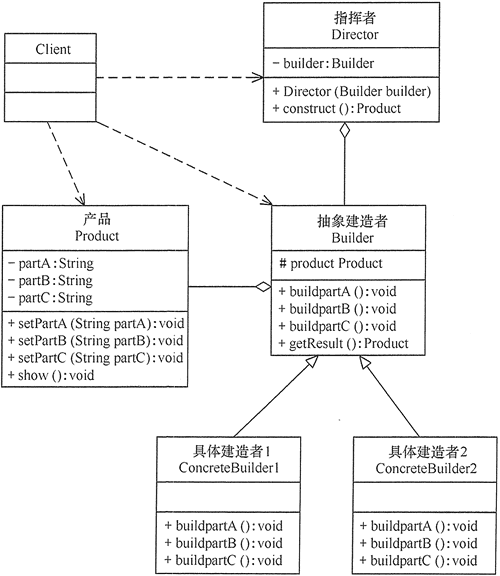
\includegraphics[width=0.8\textwidth]{image/7-1}
	\caption{建造者模式的结构图}
\end{figure}
\begin{lstlisting}
//产品角色:包含多个组成部件的复杂对象
public class Product {
	private String partA;
	private String partB;
	private String partC;
	public void setPartA(String partA) {
		this.partA = partA;
	}
	public void setPartB(String partB) {
		this.partB = partB;
	}
	public void setPartC(String partC) {
		this.partC = partC;
	}
	public void show() {
		//显示产品的特性
		System.out.println("这是产品特性");
	}
}
\end{lstlisting}
\begin{lstlisting}
//抽象建造者:包含创建产品各个子部件的抽象方法
abstract class Builder {
	//创建产品对象
	protected Product product = new Product();
	public abstract void buildPartA();
	public abstract void buildPartB();
	public abstract void buildPartC();
	//返回产品对象
	public Product getResult() {
		return product;
	}
}
\end{lstlisting}
\begin{lstlisting}
//具体建造者:实现了抽象建造者接口
public class ConcreteBuilder extends Builder {
	public void buildPartA() {
		product.setPartA("建造 PartA");
	}
	public void buildPartB() {
		product.setPartA("建造 PartB");
	}
	public void buildPartC() {
		product.setPartA("建造 PartC");
	}
}
\end{lstlisting}
\begin{lstlisting}
//指挥者:调用建造者中的方法完成复杂对象的创建
class Director {
	private Builder builder;
	public Director(Builder builder) {
		this.builder = builder;
	}
	//产品构建与组装方法
	public Product construct() {
		builder.buildPartA();
		builder.buildPartB();
		builder.buildPartC();
		return builder.getResult();
	}
}
\end{lstlisting}
\begin{lstlisting}
//客户类
public class Client {
	public static void main(String[] args) {
		Builder builder = new ConcreteBuilder();
		Director director = new Director(builder);
		Product product = director.construct();
		product.show();
	}
}
\end{lstlisting}
\section{相关设计模式}
\begin{itemize}
	\item 在Builder中,Director控制Builder,Template Method中父类控制子类;
	\item 有些Builder模式生成的实例构成了Composite模式;
	\item Builder和抽象工厂模式都用于生成复杂的实例;
	\item Builder中,Director通过组合Builder角色中的复杂方法向外部提供可以简单生成实例的接口;
	Facade模式中的Facade角色则是通过组合内部模块向外部提供可以简单调用的接口。
\end{itemize}
\section{扩展思路}
\begin{enumerate}
	\item Director不知道自己使用的究竟是Builder类的哪个子类也可以,只有不知道子类才能替换;
\end{enumerate}
